\documentclass[unicode,11pt,a4paper,oneside,numbers=endperiod,openany]{scrartcl}
\usepackage{amsmath}
\usepackage{float}  % To prevent floating of figures
\usepackage{lmodern}
\usepackage{listings}
\usepackage{hyperref}
\usepackage[utf8]{inputenc}  % Allows UTF-8 input (for special characters, etc.)
\usepackage{amsmath}         % Provides advanced math features
\usepackage{amssymb}         % For additional math symbols
\usepackage{graphicx}        % Allows including images
\usepackage{array}           % For tables
\usepackage{geometry}        % To adjust page margins
\usepackage{hyperref}        % For links and references
\usepackage{fancyhdr}        % For customized headers and footers
\usepackage{multicol}        % For multiple columns
\usepackage{verbatim}        % For verbatim text (like the gene sequence)
\usepackage{longtable}       % For long tables that span multiple pages
\usepackage{xcolor}          % For colored text (if needed)
\usepackage{listings}
\usepackage{dnaseq}         % For DNA sequences
\usepackage{amsmath}
\usepackage{float}  % To prevent floating of figures
\usepackage{lmodern}
\usepackage{listings}
\usepackage{pdfpages}

\lstset{
  language=Python,                     % Set language to Python
  basicstyle=\ttfamily\footnotesize,   % Basic font style for the code
  keywordstyle=\bfseries\color{blue},  % Keywords in bold blue
  commentstyle=\color{gray},          % Comments in green
  stringstyle=\color{orange},          % Strings in orange
  showstringspaces=false,              % Don't show spaces in strings
  frame=single,                        % Adds a frame around the code
  numbers=left,                        % Line numbers on the left
  numberstyle=\tiny\color{gray},       % Line number style
  breaklines=true,                     % Allows breaking long lines
  tabsize=4                            % Sets default tab size
}


\usepackage{ifthen}
\usepackage[utf8]{inputenc}
\usepackage{graphics}
\usepackage{graphicx}
\usepackage{hyperref}

\pagestyle{plain}
\voffset -5mm
\oddsidemargin  0mm
\evensidemargin -11mm
\marginparwidth 2cm
\marginparsep 0pt
\topmargin 0mm
\headheight 0pt
\headsep 0pt
\topskip 0pt        
\textheight 255mm
\textwidth 165mm

\newcommand{\duedate} {}
\newcommand{\setduedate}[1]{%
\renewcommand\duedate {See iCorsi for due date}}
\newcommand\isassignment {false}
\newcommand{\setassignment}{\renewcommand\isassignment {true}}
\newcommand{\ifassignment}[1]{\ifthenelse{\boolean{\isassignment}}{#1}{}}
\newcommand{\ifnotassignment}[1]{\ifthenelse{\boolean{\isassignment}}{}{#1}}

\newcommand{\assignmentpolicy}{
\begin{table}[h]
\begin{center}
\scalebox{0.8} {%
\begin{tabular}{|p{0.02cm}p{16cm}|}
\hline
&\\
\multicolumn{2}{|c|}{\Large\textbf{HPC Lab ---  Submission Instructions}}\\
\multicolumn{2}{|c|}{\large\textbf{(Please, notice that following instructions are mandatory: }}\\
\multicolumn{2}{|c|}{\large\textbf{submissions that don't comply with, won't be considered)}}\\
&\\
\textbullet & Assignments must be submitted to \href{https://www.icorsi.ch}{iCorsi} (i.e. in electronic format).\\
\textbullet & Provide both executable package and sources (e.g. C/C++ files, Matlab). 
If you are using libraries, please add them in the file. Sources must be organized in directories called:\\
\multicolumn{2}{|c|}{\textit{Project\_number\_lastname\_firstname}}\\
& and  the  file must be called:\\
\multicolumn{2}{|c|}{\textit{project\_number\_lastname\_firstname.zip}}\\
\multicolumn{2}{|c|}{\textit{project\_number\_lastname\_firstname.pdf}}\\
\textbullet &  The TAs will grade your project by reviewing your project write-up, and looking at the implementation 
                 you attempted, and benchmarking your code's performance.\\

\textbullet & You are allowed to discuss all questions with anyone you like; however: (i) your submission must list anyone you discussed problems with and (ii) you must write up your submission independently.\\
\hline
\end{tabular}
}
\end{center}
\end{table}
}
\newcommand{\punkte}[1]{\hspace{1ex}\emph{\mdseries\hfill(#1~\ifcase#1{Points}\or{Points}\else{Points}\fi)}}


\newcommand\serieheader[6]{
\thispagestyle{empty}%
\begin{flushleft}

\includegraphics[width=0.4\textwidth]{usi_inf.png}
\end{flushleft}
  \noindent%
  {\large\ignorespaces{\textbf{#1}}\hspace{\fill}\ignorespaces{ \textbf{#2}}}\\ \\%
  {\large\ignorespaces #3 \hspace{\fill}\ignorespaces #4}\\
  \noindent%
  \bigskip
  \hrule\par\bigskip\noindent%
  \bigskip {\ignorespaces {\Large{\textbf{#5}}}
  \hspace{\fill}\ignorespaces \large \ifthenelse{\boolean{\isassignment}}{\duedate}{#6}}
  \hrule\par\bigskip\noindent%  \linebreak
 }

\makeatletter
\def\enumerateMod{\ifnum \@enumdepth >3 \@toodeep\else
      \advance\@enumdepth \@ne
      \edef\@enumctr{enum\romannumeral\the\@enumdepth}\list
      {\csname label\@enumctr\endcsname}{\usecounter
        {\@enumctr}%%%? the following differs from "enumerate"
	\topsep0pt%
	\partopsep0pt%
	\itemsep0pt%
	\def\makelabel##1{\hss\llap{##1}}}\fi}
\let\endenumerateMod =\endlist
\makeatother




\usepackage{textcomp}





\begin{document}



\setassignment

\serieheader{High-Performance Computing Lab}{Institute of Computing}{Student: Jonatan Bella}{Discussed with: NONE}{Solution for Project 2}{}
\newline

\assignmentpolicy
This project will introduce you to parallel programming using OpenMP. 

\section{Parallel reduction operations using OpenMP \punkte{20}}
\subsubsection{Reduction and Critical}
First, each implementation have an outer loop with the number of iterations ($NUM\_ITERATIONS$) since we used for benchmarking by running
the repeated dot products. 
Now, on the case of the reduction, the inner loop that contains the actual dot product implementation needs a specified pragma 
for parallelizing the loop operation with Open MP. The pragma is as follows:
\begin{lstlisting}
#pragma omp parallel for reduction(+:alpha_parallel)
\end{lstlisting}
Where we specified the directive to parallelize the for loop ($\#pragma\ omp\ parallel\ for$) and the reduction operation 
($reduction(+:alpha\_parallel)$) that will be performed on the variable $alpha\_parallel$. Notice that we could have also set $default(none)$, but
that would have required us to set the shared variables (a, b) which is done by default in OpenMP. -Any variables that existed before a parallel region still exist inside, and are by
default shared between all threads"- \footnote{ 6.1.2 Introduction to High Performance Computing for Scientists and Engineers by Georg Hager and Gerhard Wellein}.
The reductions automatically privatizes the specified variable ($alpha\_parallel$) and at the end the value of the variable is reduced to a single value into the shared instance of the variable 
using the specified operation ($+$ in this case) to get the final result. 

\begin{lstlisting}
    for (int iterations = 0; iterations < NUM_ITERATIONS; iterations++) {
        alpha_parallel = 0.0;
        #pragma omp parallel for reduction(+:alpha_parallel)
        for (int i = 0; i < N; i++) {
          alpha_parallel += a[i] * b[i];
        }
      }
\end{lstlisting}

or \footnote{I implemented both scenarios to check if there is a difference in the results, or if the precision of the final sum changes somehow.
I used the first form for the scaling analysis plot since there is no significant change. The other graph can be found on the code - dotProduct - exe1-0-2 - defaultNoneCase}:

\begin{lstlisting}
    for (int iterations = 0; iterations < NUM_ITERATIONS; iterations++) {
        alpha_parallel = 0.0;
        #pragma omp parallel for default(none) shared(a, b, N) reduction(+:alpha_parallel)
        for (int i = 0; i < N; i++) {
          alpha_parallel += a[i] * b[i];
        }
      }
\end{lstlisting}

In the other hand, for the critical implementation, we need to create first the parallel region defined by:
\begin{lstlisting}
#pragma omp parallel
\end{lstlisting}
After that, we declare a $local_sum$ variable inside the parallel region which sets the local sum for each thread (therefore, each thread has its own copy). 
Then, we need to specify the type of parallelization, which in this case is a for loop that will distribute the loop iterations among the threads with a and b shared.
And the critical region that will be executed by only one thread at a time. This allows us to only use the critical section only in the specific integration of the thread where the race 
condition can arise. Critical regions solve this problem assuring that most one thread at a time executes that piece of code. \footnote{ Based on chapter 6 of introduction to High Performance Computing for Scientists and Engineers by Georg Hager and Gerhard Wellein,
email from Daniel Sergio Vega Rodríguez}
\begin{lstlisting}
for (int iterations = 0; iterations < NUM_ITERATIONS; iterations++) {
    alpha_parallel = 0.0;
    #pragma omp parallel
    {
        long double local_sum = 0.0; //each thread local sum
        #pragma omp for
        for (int i = 0; i < N; i++) {
        local_sum += a[i] * b[i];
        }
        //then we add them all together
        #pragma omp critical
        {
        alpha_parallel += local_sum;
        }
    }
    }
\end{lstlisting}

or \footnote{Notice here that I used a different variable, so I could store the alpha values
of the different implementations for the next section of the questions.}: 

\begin{lstlisting}
    for (int iterations = 0; iterations < NUM_ITERATIONS; iterations++) {
        alpha_parallel_critical = 0.0;
        #pragma omp parallel default(none) shared(a, b, N, alpha_parallel_critical)
        {
          long double local_sum = 0.0; //each thread local sum
          #pragma omp for
          for (int i = 0; i < N; i++) {
            local_sum += a[i] * b[i];
          }
          //then we add them all together
          #pragma omp critical
          {
            alpha_parallel_critical += local_sum;
          }
        }
      }
\end{lstlisting}

The time is measure on each case as specified with the following results: 

\begin{figure}[H]
    \centering
    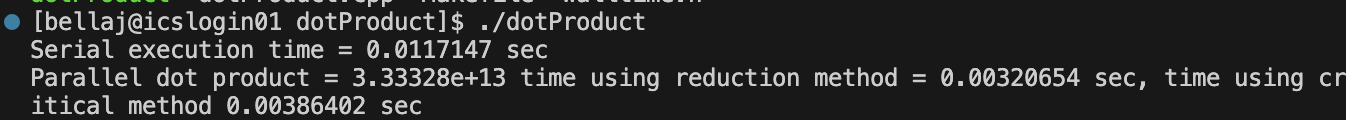
\includegraphics[width=\textwidth]{./img/exe1/image.png}
    \caption{Example result with N = 100000}
\end{figure}

\subsubsection{Scaling analysis on Rosa Cluster}
To solve this exercise, I first centralize the outputs of the different implementations in one line \footnote{I leave commented the given commands in case is needed for correction with some additional comments on the sources 
used for the implementation.}:

\begin{lstlisting}
    printf("%d %d %.6f %.6f %.6f %.10Lf %.10Lf %.10Lf\n", N, omp_get_max_threads(), time_serial, time_red, time_critical, alpha_parallel,alpha_parallel_critical, alpha);
\end{lstlisting}

With the idea of storing in a ".data" file as it was done on the previous assignment for benchmarking. 
Notice that I store the different data sizes, the number of threads, the time for the serial implementation, the time for the reduction implementation, the time for the critical implementation, 
the result of the reduction implementation, the result of the critical implementation and the result of the serial implementation.
In addition, I added a line for receiving the N value as argument, since the ideas is to run a loop with different N and threads values from the bash file. 

\begin{lstlisting}
    int N = atoi(argv[1]);
\end{lstlisting}

Then, I created the bash file also following a similar pattern to the $run\_matrixmult.sh$ file from the previous assignment.
Where first I define the batch configurations, load the modules, define a list of N and threads elements to be loop over; 
calculating the respective dot products for each thread given N with $export \ OMP\_NUM\_THREADS=\$T$, and for each N, storing the results in a ".data" file. 
\footnote{https://stackoverflow.com/questions/11162406/open-and-write-data-to-text-file-using-bash} 

In addition, I tried to generate the graph directly with gnuplot however, I was not able to add a legend with the different N values. Therefore, I did it with a python script using the .data file. 

\begin{figure}[H]
    \centering
    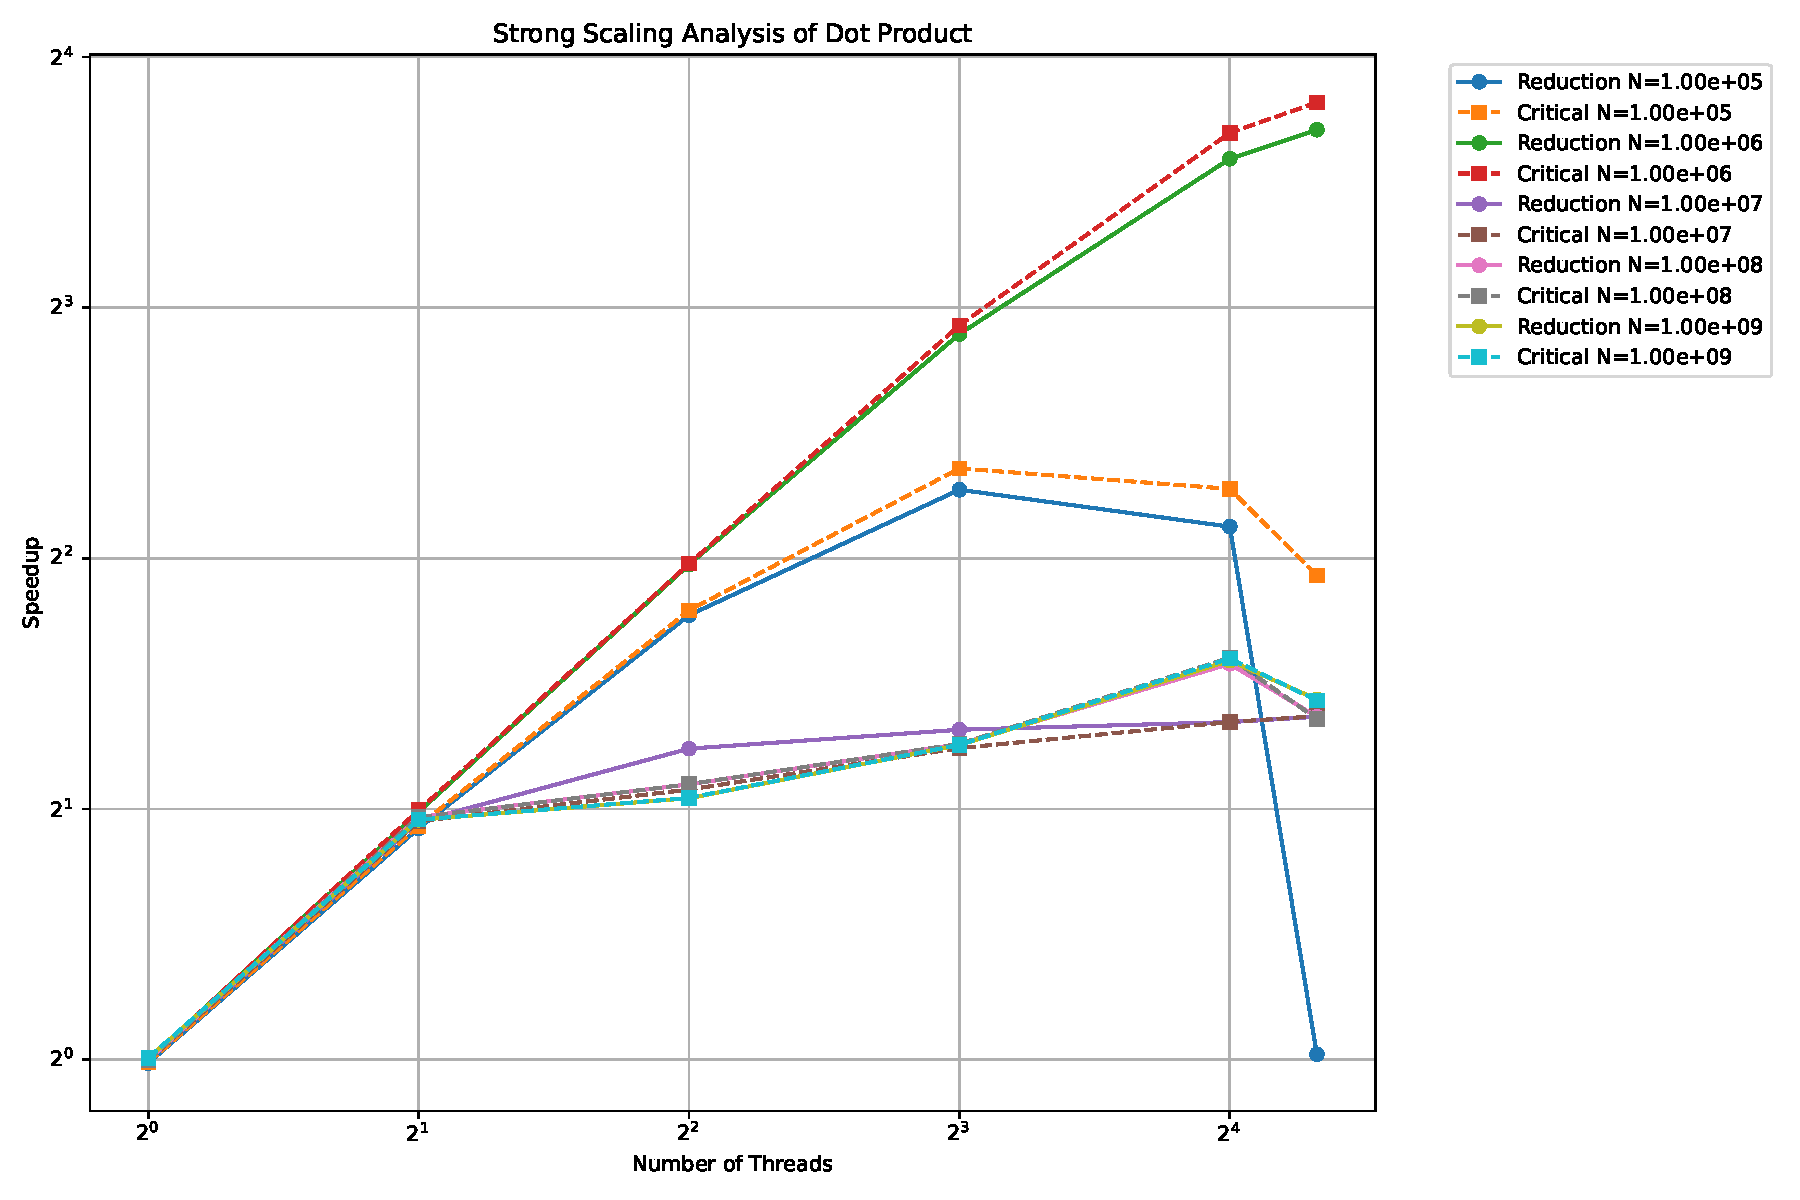
\includegraphics[width=\textwidth]{./img/exe1/dotproduct_strong_scaling.pdf}
    \caption{Strong scaling analysis}
\end{figure}

Each curve of the graph is a ratio of the time of the serial implementation over the time of the parallel implementation, where each color 
indicates a different N value and implementation (critical and reduction). In case of strong scaling, 
the number of processors, in this case of threads, is increased while the problem size (N) remains constant.\footnote{https://hpc-wiki.info/hpc/Scaling}

I was expecting that the performance increase when higher N gets, since it will "dilute" the overhead cost of the parallelization. 
This occurs from $10^5$ to $10^6$ where the performance is better for the parallel implementations, however, things get relatively worse for higher N values.
Of course, the parallelization performance is superior to the single threaded one, but the gain is relatively less when the N value is higher than $10^6$ and i think the 
reason for this lies on memory utilization as we discussed on previous assignment.

If we store the a and b vectors as doubles then N = $10^5$ will require 1.6 MB of memory (2 *  8 * $10^5$). 
Then, for N = $10^6$ we will need 16 MB of memory and for N = $10^7$ we will need 160 MB of memory. Now, our L3 memory in 
Rosa cluster has 25 MB of memory, therefore, from N = $10^6$ we will start to have memory issues, and that could be impacting the threads gain 
and explain why we get the expected gain in performance when N = $10^5$ and $10^6$ but not for higher values.

With respect to the difference between the critical and reduction implementations, I do not see a substantial difference between each other. 
Surprisingly, the critical implementation is slightly faster than the reduction implementation which is not what I expected since the reduction seems to be 
particularly designed for these cases \footnote{Based on main book comments about both on chapter 6}. Maybe there is some overhead in the reduction implementation 
that is not present in the critical implementation, although, the difference is too small to conclude about it.

\subsubsection{Parallel Efficiency}

To calculate the parallel efficiency we need to obtain the ratio between the speedup before calculated and the number of threads used. \footnote{\url{https://cvw.cac.cornell.edu/parallel/efficiency/about-efficiency}}

\begin{align*}
    Parallel_Efficiency = \frac{Speedup}{number\_of\_threads}
\end{align*}

\begin{figure}[H]
    \centering
    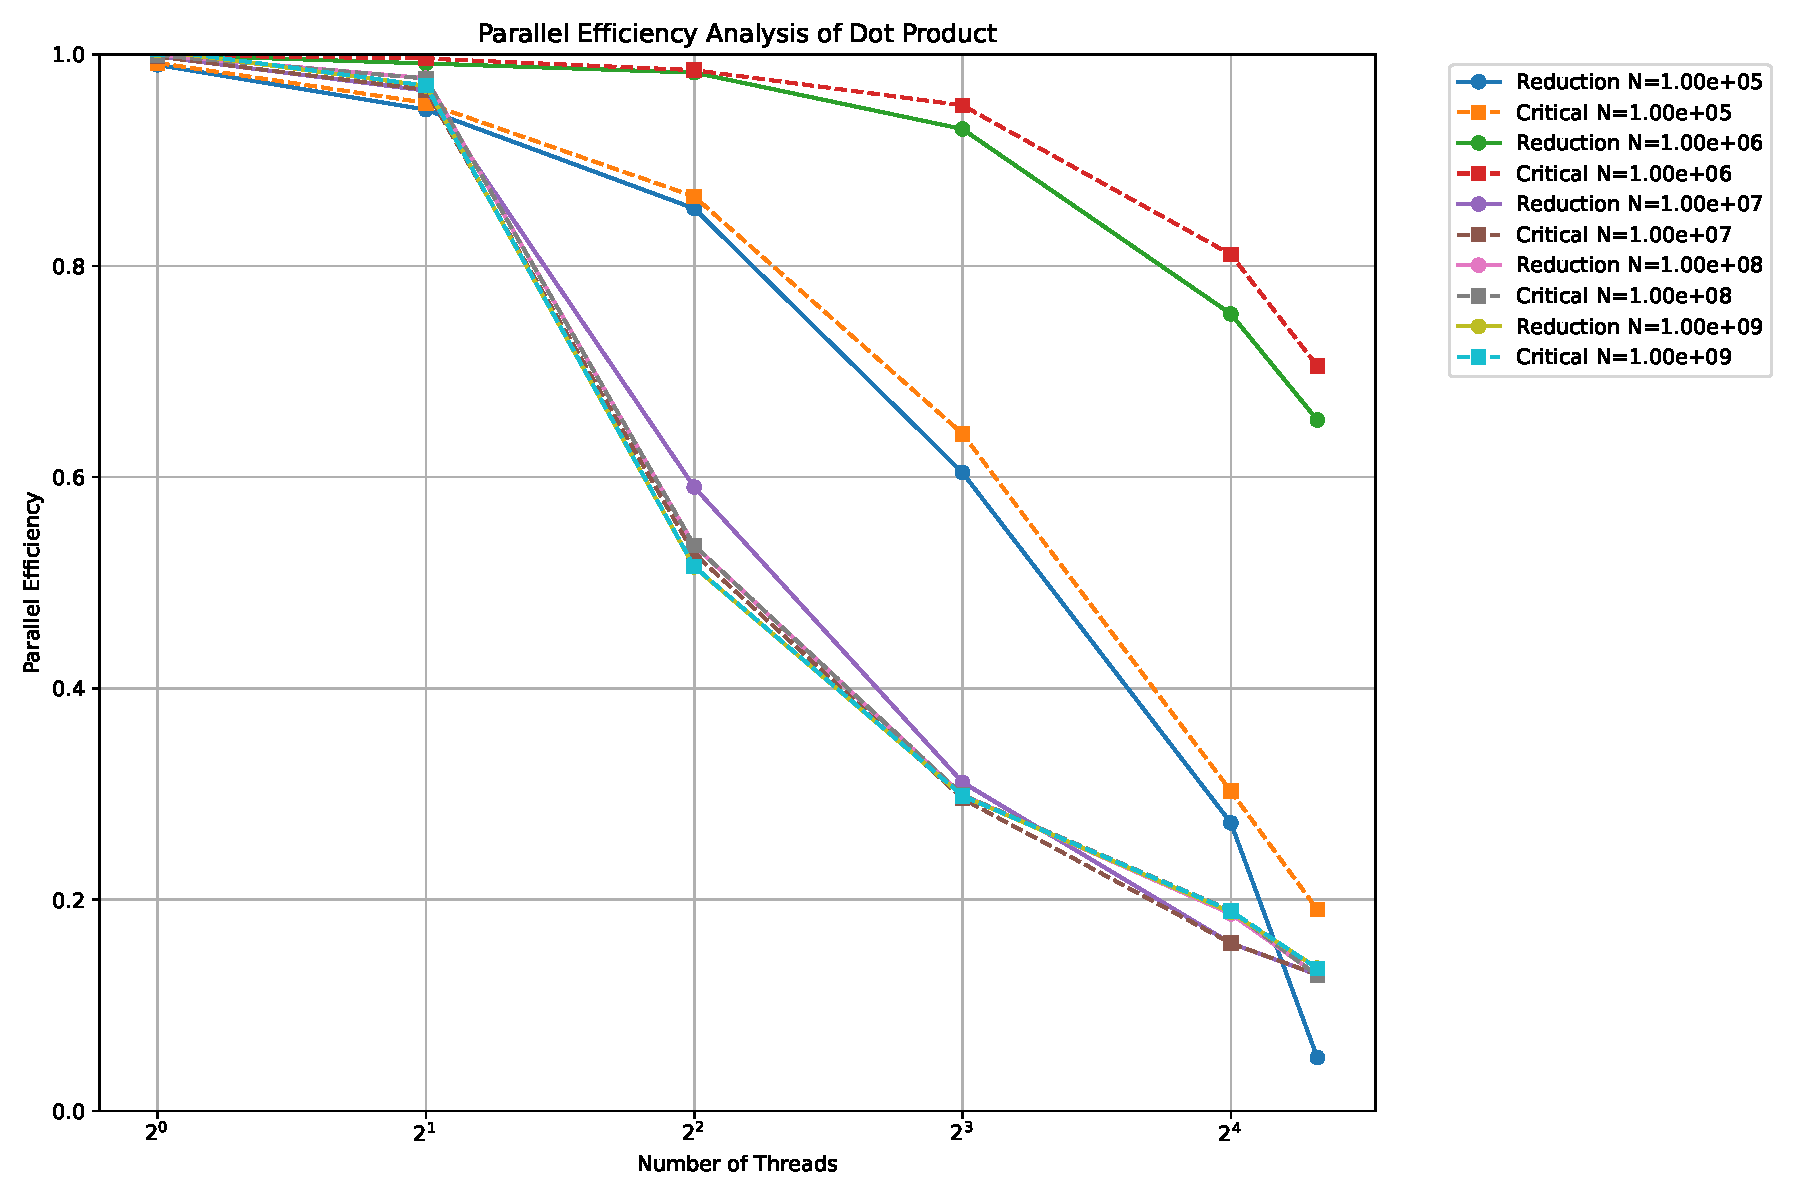
\includegraphics[width=\textwidth]{./img/exe1/dotproduct_parallel_efficiency.pdf}
    \caption{Parallel efficiency}
\end{figure}

As before, we have this general improvement because of parallelization, especially until N = $10^6$, right before the L3 memory limit is reached (as explained in the previous point).
Now, we can see that is not exactly linear \footnote{\url{https://hpc-wiki.info/hpc/Scaling} 
\newline \url{https://waterprogramming.wordpress.com/2021/06/07/scaling-experiments-how-to-measure-the-performance-of-parallel-code-on-hpc-systems/}
\newline \url{https://scicomp.ethz.ch/wiki/Parallel_efficiency}}, 
the Amdahl's law implies a limit on how much faster you can solve a problem by using additional cores -"the overall performance improvement gained by optimizing a single part of a system
is limited by the fraction of time that the improved part is actually used"- \footnote{Amdahl's wikipedia}. What Amdahl states here is that the importance 
of the serial - non parallelize - fraction of the code acquires more importance as more efficiently the parallelize fraction is managed:
\begin{align*}
    Speedup &= \frac{serial\_runtime}{parallel\_runtime} \\
    &= \frac{F_s + F_p}{F_s + F_p/N} \\
    &= \frac{1}{F_s + F_p/N} \\
    \lim_{N \to \infty} Speedup &= \frac{1}{F_s}
\end{align*}

where:
\begin{itemize}
    \item $serial\_runtime$ is the execution time of the program running on a single processor
    \item $parallel\_runtime$ is the execution time of the program running on $N$ parallel processors
    \item $F_s$ is the fraction of the serial implementation.
    \item $F_p$ is the fraction of the program that can be parallelized ($F_s + F_p = 1$)
    \item $N$ is the number of processors (or threads) used in the parallel execution
\end{itemize}

Therefore, the single threaded part of the codes form an asymptote for the performance of the parallelize code which 
explains the concave look of the curves when threads are increased. Notice that this is accentuated by the memory bandwidth limit that we discussed before.

In general, two threads for any N value seems to provide a substantial gain in performance, however, for higher threads the gain is substantial for N until $10^6$, and then the relative increase in 
performance reduces. In addition, the critical implementation seems to be slightly better than the reduction implementation. 
\subsection{Approximating PI}
To implement the pi approximation, I first created the function $f$ that should be evaluated on each iterative step. 

\begin{lstlisting}
    double f(double x) {
        return 4.0 / (1.0 + x * x);
    }
\end{lstlisting}

Then, for the simple approximation, we can think of the area calculation problem as creating small cuts on the function of width $dx$ with height $f(x)$ and summing all the areas of the rectangles.
Therefore, we compute the centers of the interval $x_i$ as provided and evaluate in $f$ for each iteration of the interval. We can take the $dx$ as common factor since all the intervals are the same size.
We take into account that the size of N can be over the size of int, therefore, we use a long int for the loop.
\begin{lstlisting}
    for (long int i = 0; i < N; i++) {
        double x = (i + 0.5) * dx; 
        sum += f(x);
    }
\end{lstlisting}

For the parallel implementation, I choose to use the reduction since it is more elegant and cleaner.

\begin{lstlisting}
    #pragma omp parallel for reduction(+:sum)
    for (long int i = 0; i < N; i++) {
        double x = (i + 0.5) * dx;
        sum += f(x);
    }
\end{lstlisting}
As on previous exercise, the implementation is as simple as adding the specific directive for the for loop 
parallelization and the reduction operation with the target variable to privatize.

\begin{figure}[H]
    \centering
    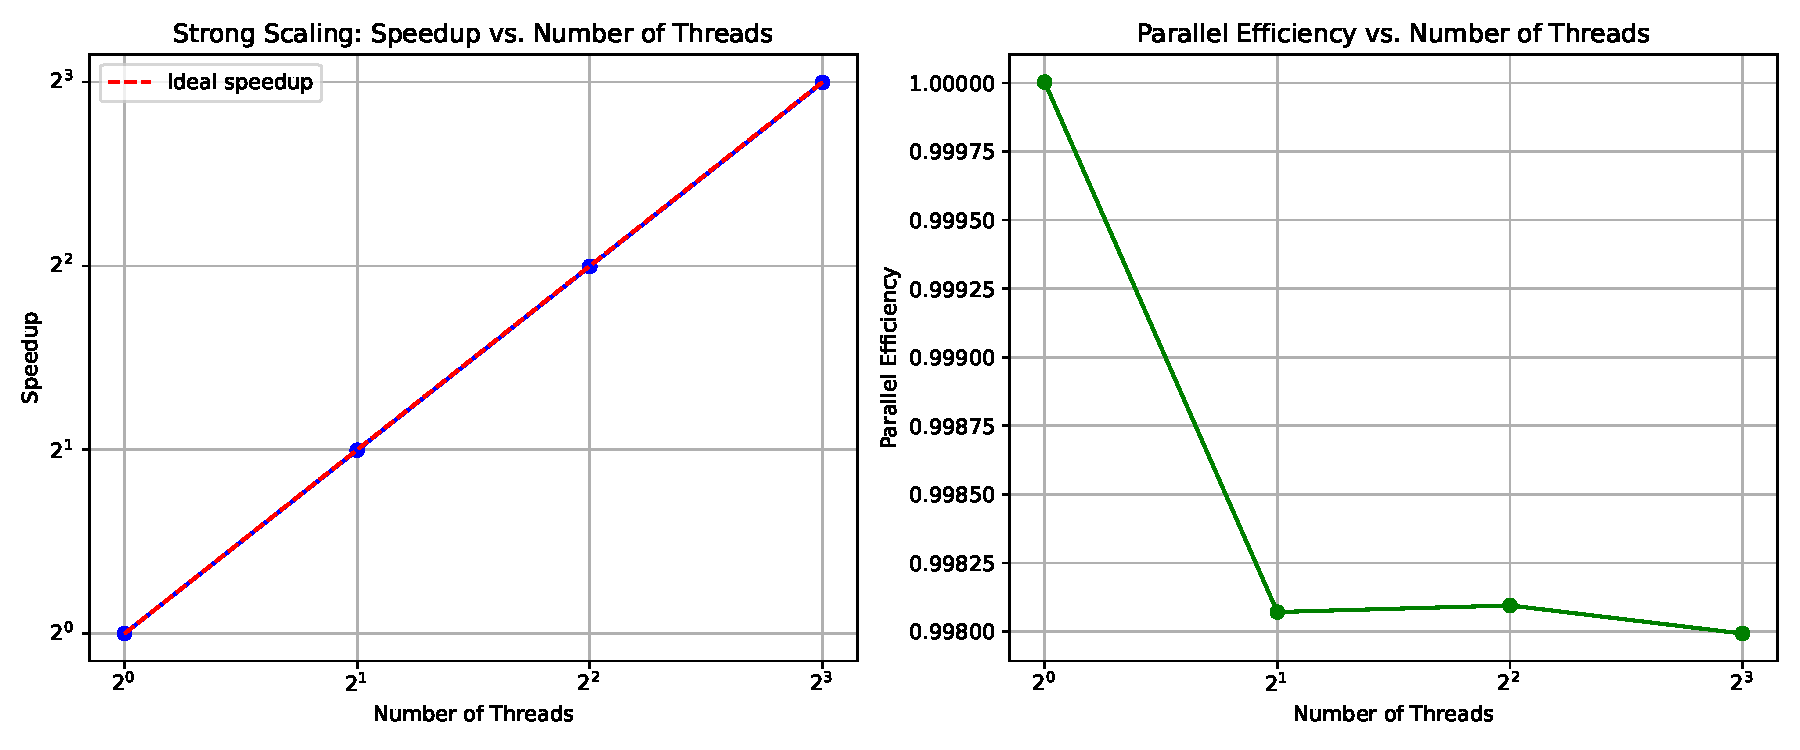
\includegraphics[width=\textwidth]{./img/exe1/pi_approximation_plots.pdf}
    \caption{Strong scaling analysis and Parallel efficiency for pi approximation}
\end{figure}

The gains from parallelization follow the ideal speedup which indicates that the parallelization is well done.
As explained before, the speedup is defined as the ratio of the execution time of the serial algorithm vs 
the parallel algorithm. Strong Scaling then refers to how the solution varies with the number of threads keeping 
N constant on $10^9$ in this case. In the plot we can see how this behavior benefits perfectly from scaling without suffering 
from Amdahl's law since the serial part of the code is minimal.

The parallel efficiency is also then close to 1 for all the number of threads, which indicates that the processors are well utilized.
Meaning that the overhead is minimal, and the workload is well-balanced. This result is clearly related with strong scaling one since 
a perfect strong scaling will indicate a speedup equal to the number of threads which would set the parallel efficiency ratio in 1 
for each thread. Therefore, the results are almost perfect at least until 8 threads for this problem.

\section{The Mandelbrot set using OpenMP \punkte{20}}
The Mandelbrot set is composed of those complex numbers $c$ for which the function $f_c(z) = z^2 + c$ does not diverge when iterated from $z = 0$.
Which can be shown to be those values of $c$ where no term of the iteration is at a distance greater than 2 from the origin.
Therefore, we want to check if after a sufficient amount of iteration we stay within the 2 unit circle of the complex plane. If in any
case we go out of this circle, we can say that the point is not part of the Mandelbrot set.\footnote{I watched the 
following videos to remind me about more details of the Mandelbrot set:
    \url{https://www.youtube.com/watch?v=FFftmWSzgmk}
    \newline \url{https://www.youtube.com/watch?v=NGMRB4O922I}
    \newline \url{https://www.youtube.com/watch?v=oCkQ7WK7vuY}
}

\begin{lstlisting}
    while (x2 + y2 < 4.0 && n < MAX_ITERS) { 
        y = 2 * x * y + cy;
        x = x2 - y2 + cx;
        x2 = x * x;
        y2 = y * y;
        n++;
        }
\end{lstlisting}

If x is the real term of the complex number and y the imaginary part:
\begin{align*}
    |z| &= |x + yi| \\
    &= \sqrt{x^2 + y^2}
\end{align*} 

Then, to be part of the unit 2 circle:

\begin{align*}
    \sqrt{x^2 + y^2} &< 2 \\
x^2 + y^2 &< 4
\end{align*} 

Now, for evaluating again, we need to update the proper value of the real and imaginary part:

\begin{align*}
    z^2 &= (x + yi)(x + yi) \\
    &= x^2 - y^2 + 2yxi 
\end{align*} 

Since $f$ is $f_c(z) = z^2 + c$. 
The real term of the new iteration of the expression:
\begin{align*}
    x &= x^2 - y^2 + cx \\
\end{align*} 
where $x^2 - y^2$ are the real term of $z^2$ and $cx$ the real term of the constant

The imaginary term: 
\begin{align*}
    y &=  (2yx + cy)i \\
\end{align*}

To keep track of the iterations we need a counter the accumulates n. therefore, after the while loop i added: 

\begin{lstlisting}
    nTotalIterationsCount += n;
\end{lstlisting}

As required by the exercise. Notice that many values will finish interrupt the while loop much before than others, 
which will probably make the load of the loop more dynamic than static computations.

Finally, with respect to the parallelization there are many ways to actually implement it. 
I first tried with using simply a reduction operation on the nTotalIterationsCount variable by 
adding a pragma directive on the outer loop. However, this does not work since the final image will be distorted
(even after setting all variables private). 

Therefore, I realize that it is necessary to find a way to take care of the image processing part. 
\footnote{Besides the presented option, it could be possible to create a buffer holding the image 
iteration values that then, outside the parallelize loop, we used to create the image with the provided 
function. The probable advantage would be that the buffer is parallelizable, however, I use the critical section
as presented here. }

For this, we could add a critical section around the image 
code ($png\_plot$) to ensure that only one thread is writing to the image at a time:

\begin{lstlisting}
#pragma omp parallel reduction(+:nTotalIterationsCount) private(x, y, x2, y2, cx, cy, i)
{
    #pragma omp for schedule(dynamic)
    for (j = 0; j < IMAGE_HEIGHT; j++) {
        cy = MIN_Y + j * fDeltaY;
        for (i = 0; i < IMAGE_WIDTH; i++) {
            cx = MIN_X + i * fDeltaX;
            x = cx;
            y = cy;
            x2 = x * x;
            y2 = y * y;
            int n = 0;
            while (x2 + y2 < 4.0 && n < MAX_ITERS) { 
            y = 2 * x * y + cy;
            x = x2 - y2 + cx;
            x2 = x * x;
            y2 = y * y;
            n++;
            }
            nTotalIterationsCount += n;
            int c = ((long)n * 255) / MAX_ITERS;
            #pragma omp critical
            {
            png_plot(pPng, i, j, c, c, c);
            }
        }
    }
}
\end{lstlisting}

To implement this, I first create the threads where each of them will have its own private copy of x,y,$x^2$,$y^2$,cx,cy and adding a reduction 
clause on the $nTotalIterationsCount$ variable such that it also create a local copy for each thread that gets aggregate at the end to avoid 
a race condition. Now, the outer loop is parallelized with the $omp for$ directive and I add the schedule dynamic (I tried static and dynamic, but I stayed with dynamic mostly 
because, as I mentioned before, makes more sense according to the problem we have where we do not know before what set of values will explode).
Most importantly, I wrap the $png_plot$ function with a critical section to ensure that only one thread at a time write to the image, to avoid 
the distortion of the image as I mentioned before with the simple reduction operation. Therefore, the parallelization is done over the rows of the image
(j loop) and each thread computes a subset of those rows independently. 

It is also important to add the corresponding flags to the makefile to compile the program with the OpenMP library:

\begin{lstlisting}
all: mandel_seq

mandel_seq: mandel_seq.o pngwriter.o walltime.o
    gcc -O3 -fopenmp -o mandel_seq mandel_seq.o pngwriter.o walltime.o -lpng

mandel_seq.o: mandel_seq.c consts.h pngwriter.h walltime.h
    gcc -O3 -fopenmp -c mandel_seq.c

pngwriter.o: pngwriter.c pngwriter.h
    gcc -O3 -fopenmp -c pngwriter.c

walltime.o: walltime.c walltime.h
    gcc -O3 -fopenmp -c walltime.c

clean:
    rm -f *.o mandel_seq

.PHONY: all clean
\end{lstlisting}

Since i could not make it work straight forwardly with the provided code for the makefile, i based most of my construction from 
a makefile tutorial website, previous exercises makefile , and a medium post with makefile basics \footnote{\url{https://makefiletutorial.com}
\newline
\url{https://medium.com/@ayogun/makefile-basics-beginner-intermediate-c92377542c2c}}.
Where $all:$ is the target that will be executed, mandel\_seq is the executable that will be created, and the dependencies are the object files that are needed to create the executable. 
Then, the commands to compile the object files and the executable are specified with the corresponding 
openmp flag. Finally, the clean target is defined to remove the object files and the executable.

In addition to this, I create a bash file following the same structure that on previous exercise: 
\begin{lstlisting}
#!/bin/bash
#SBATCH --job-name=Mandel
#SBATCH --output=Mandel-%j.out
#SBATCH --error=Mandel-%j.err
#SBATCH --ntasks=1
#SBATCH --cpus-per-task=20
#SBATCH --partition=slim
#SBATCH --time=04:00:00

module load gcc
module list
make

thread=(1 2 4 8 16 20)

#we intialize the files we need
data_file="mandelbrot_results.data"
full_output_file="mandelbrot_full_output.txt"
echo "# Threads Total_Time Iterations_per_Second MFlops" > $data_file
> $full_output_file

for T in "${thread[@]}"; do
    echo "Running with T = $T threads" | tee -a $full_output_file
    export OMP_NUM_THREADS=$T
    
    # the full output if required
    output=$(./mandel_seq | tee -a $full_output_file)
    echo "----------------------------------------" >> $full_output_file
    
    #for our .data
    total_time=$(echo "$output" | grep "Total time:" | awk '{print $3}')
    iterations_per_second=$(echo "$output" | grep "Iterations/second:" | awk '{print $2}')
    mflops=$(echo "$output" | grep "MFlop/s:" | awk '{print $2}')
    echo "$T $total_time $iterations_per_second $mflops" >> $data_file
done
gnuplot mandelplot.gp
\end{lstlisting}

The main difference is that I made use of AWK to extract only the numbers from the string output of the program.
This works by first storing the output of the program in a variable, then using grep to filter the lines 
that contain the specific string that we are interested in, and finally using AWK to extract the number from the string.
\footnote{
    \url{https://www.adamcouch.co.uk/awk-part-1/}
    \newline \url{https://stackoverflow.com/questions/10992814/passing-grep-into-a-variable-in-bash}
}
I did this to be able to use the same it was done on the previous assignment with benchmarking:
\begin{lstlisting}
set terminal png size 800,600
set output 'mandelbrot_performance.png'
set title 'Mandelbrot Set Performance'
set xlabel 'Number of Threads'
set ylabel 'Performance'
set key outside
set logscale x 2
plot 'mandelbrot_results.data' using 1:4 with linespoints title 'MFlop/s'
\end{lstlisting}
To plot automatically the results of the program, using the same structure as before.
\footnote{Source for this was the timing.gp of previous assignment 
\newline and
\url{https://ctcms-uq.github.io/data_tutorials/gnuplot.html}}

In addition, I made use of tee as on the previous assignment bash file, to accumulate (-a) the whole output of the program in a file.
This returns us with the whole prints that were created with a more detailed statistics: 

\begin{table}[h]
\centering
\small
\begin{tabular}{|c|c|c|c|c|c|}
\hline
\textbf{Threads} & \textbf{Time (s)} & \textbf{Time/pixel} & \textbf{Time/iter} & \textbf{Iter/s} & \textbf{MFlop/s} \\
\hline
1 & 156.079 & 9.30e-06 & 4.83e-09 & 2.07e+08 & 1658 \\
2 & 79.629 & 4.75e-06 & 2.46e-09 & 4.06e+08 & 3250 \\
4 & 40.139 & 2.39e-06 & 1.24e-09 & 8.06e+08 & 6447 \\
8 & 21.196 & 1.26e-06 & 6.55e-10 & 1.53e+09 & 12208 \\
16 & 11.699 & 6.97e-07 & 3.62e-10 & 2.76e+09 & 22119 \\
20 & 9.935 & 5.92e-07 & 3.07e-10 & 3.26e+09 & 26047 \\
\hline
\end{tabular}
\caption{Mandelbrot set computation performance with varying thread counts}
\label{tab:mandelbrot_perf}
\end{table}

As the number of threads increases the execution time decreases, which is a good 
sign for our parallelization. As we can see on figure 6, the strong scaling shows a substantial
speedup that is almost ideal (15.71 times faster for 20 threads - ideal would be 20). 
The parallel efficiency at 20 threads is around $78.56\%$ which is a good core utilization 
but not perfect, as we discussed with the Amdahl's law. The iterations per second and 
the MFlop/s also reflect the improvement. 

Since the problem is not perfectly parallelizable given the plotting of the image,
we can see those diminishing returns. 


\begin{figure}[H]
    \centering
    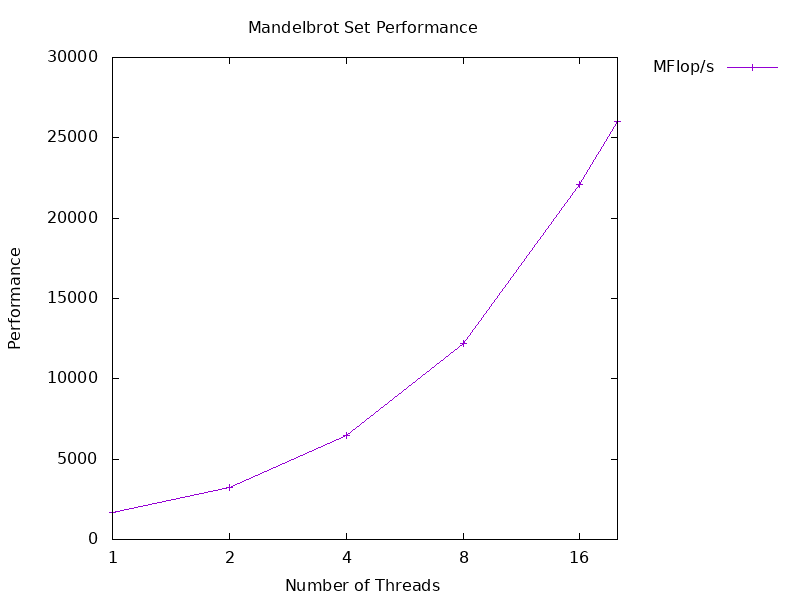
\includegraphics[width=\textwidth]{./img/exe2/mandelbrot_performance.png}
    \caption{MFlop/s with respect to the number of threads}
\end{figure}

\begin{figure}[H]
    \centering
    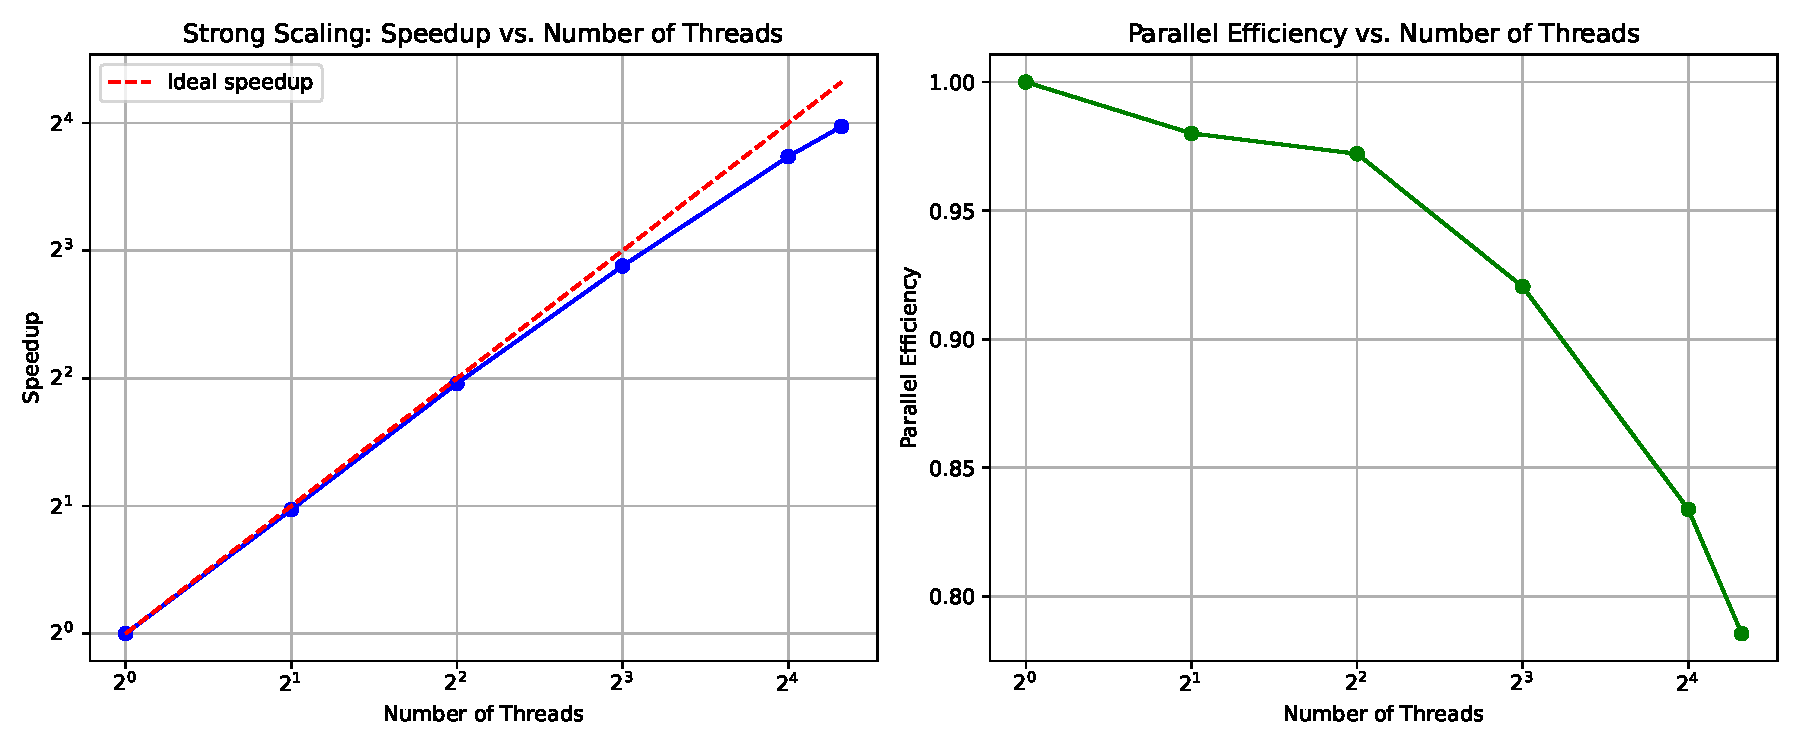
\includegraphics[width=\textwidth]{./img/exe2/mandel_plot.pdf}
    \caption{Strong Scaling and Parallel Efficiency}
\end{figure}

\begin{figure}[H]
    \centering
    
\includegraphics[width=0.9\textwidth]{./img/exe2/mandel.png}
    \caption{The beautiful Mandelbrot set}
\end{figure}

\section{Bug hunt \punkte{15}}
\subsection{Bug 1}
For this first case the problem is that 
this will not even run since it is necessary to apply the pragma directives to the for loop itself;
wrapping the for loop with "\{" "\}" will not work since the for directive already applies to the for
loop itself. 
\subsection{Bug 2}
First, the total variable is defined outside the parallel section. However, many threads 
will be writing on it in the for directive parallelization section. To solve this we could add a
$reduction(+:total)$ clause to the pragma directive.
Another thing that can be considered as a mistake is that the $tid$ variable is defined inside the parallel
region, but the related print is outside it. Which means that it will print out 0, the last - main -  thread it was used, if that
is the objective then it is fine, but if the objective is to print each thread id then it should be inside the parallelized region.
\subsection{Bug 3}
One main problem here is a deadlock problem that emerge from the barrier usage in the $print_results$ function. 
Basically, with the omp sections directive we create two separate sections that are executed by two different threads (if available). 
Now, both call the $print_results$ function that have inside a barrier directive. 
This barrier directive requires that all threads reach it before any can proceed. 
Therefore, if we only have 1 or 2 threads, that works. But if we have more than two
then, thread 1 reach the barriers and wait, the second one also reaches it and waits, but the rest
will never reach that because they are not executing that function which will make an infinite wait. 
\subsection{Bug 4}
As soon as trying to run it, you get back "Segmentation fault (core dumped)" which happens when any program
tries to access a part of memory that is not allowed to access.\footnote{https://www.naukri.com/code360/library/segmentation-fault-in-cpp}
This happens when a program tries to access an out of bound memory location, when tries to write in a read only memory or that it was not allocated yet. 

In this case, we have a large matrix of NxN that is made private on parallelization. Now, N = 1048, then $n*n$ =  8.38 MB.
Since a is declared in the main function, is allocated on the stack. The parallelization makes $a$ private for each thread.
However, the maximum stack size is 8MB for linux distros \footnote{\url{https://softwareengineering.stackexchange.com/questions/310658/how-much-stack-usage-is-too-much}} 
Each thread trying to allocate this local variable will cause the stack to overflow and the program to crash.
To solve this, we could increase the stuck size, but it is not scalable to the number of threads that can vary \footnote{Environment variables - 6.1 - main book chapter}
Or we could make use of dynamic memory (heap) to allocate the matrix, allocating the memory during runtime.
\subsection{Bug 5}
The problem that can emerge here is that after the barrier, when all the threads are synchronized, there are two sections run by 
two different threads. The first one set a lock on $locka$ and proceed to initialize a, then it tries to acquire b, so it can add a with b. 
However, at the same time, the second thread lockb and then initialize b, the problem now is that it tries to acquire locka to add b with a. 
therefore, we can end up in a deadlock since thread one acquired locka and is waiting for lockb to complete the addition, but the second thread already acquire 
lockb and is waiting for locka to complete the addition. This is circular since both are holding a lock on what the other needs at the same time.
\section{Parallel histogram calculation using OpenMP \punkte{15}}
I will first make a brief explanation of false sharing and how it applies in this case. 
False sharing, as stated in the book, is a performance issue that occurs when there is a parallel computation 
ongoing using shared memory such that each core has its own cache, data is transferred between the main memory 
and the cache in fixed-sized cache lines, and when we have multiple threads frequently modifying variables that are independent 
but located in the same cache line then the thread that did the modification causes that the other threads need to reload the cache line.
The other threads could be using an element of the cache line, that's why they need to reload, even if the element they need is not the one updated. 
This leads to an increase in cache data traffic which can increasingly degrade performance with more threads. 

For example, in the case of the histogram, where each thread updates its own element in an array, if these elements are 
close enough to share a cache line then a false sharing may occur. So it is "false sharing" since they share a cache line but not
the actual data. The authors propose padding (that adds extra space between variables, so they don't share cache lines) or/and privatization - that gives each
thread its own copy of the data structure -.

In this case, I will create a local variable in the parallelization such that each thread has its own copy of the histogram. 
Then, at the end, I will add the local histograms to the global histogram.

\begin{lstlisting}
    #pragma omp parallel
    {
      long dist_private[BINS] = {0};  
  
      #pragma omp for
      for (long i = 0; i < VEC_SIZE; ++i) {
        dist_private[vec[i]]++;
      }
  
      #pragma omp critical
      {
        for (int i = 0; i < BINS; ++i) {
          dist[i] += dist_private[i];
        }
      }
    }
\end{lstlisting}

As you can see, the idea was to create a local histogram for each thread, each of them adding the
corresponding values to the local histogram. Then, at the end, we add the local histograms to the global histogram with 
the critical clause to avoid race condition on the sum. 

The results are the following: 
\begin{figure}[H]
    \centering
    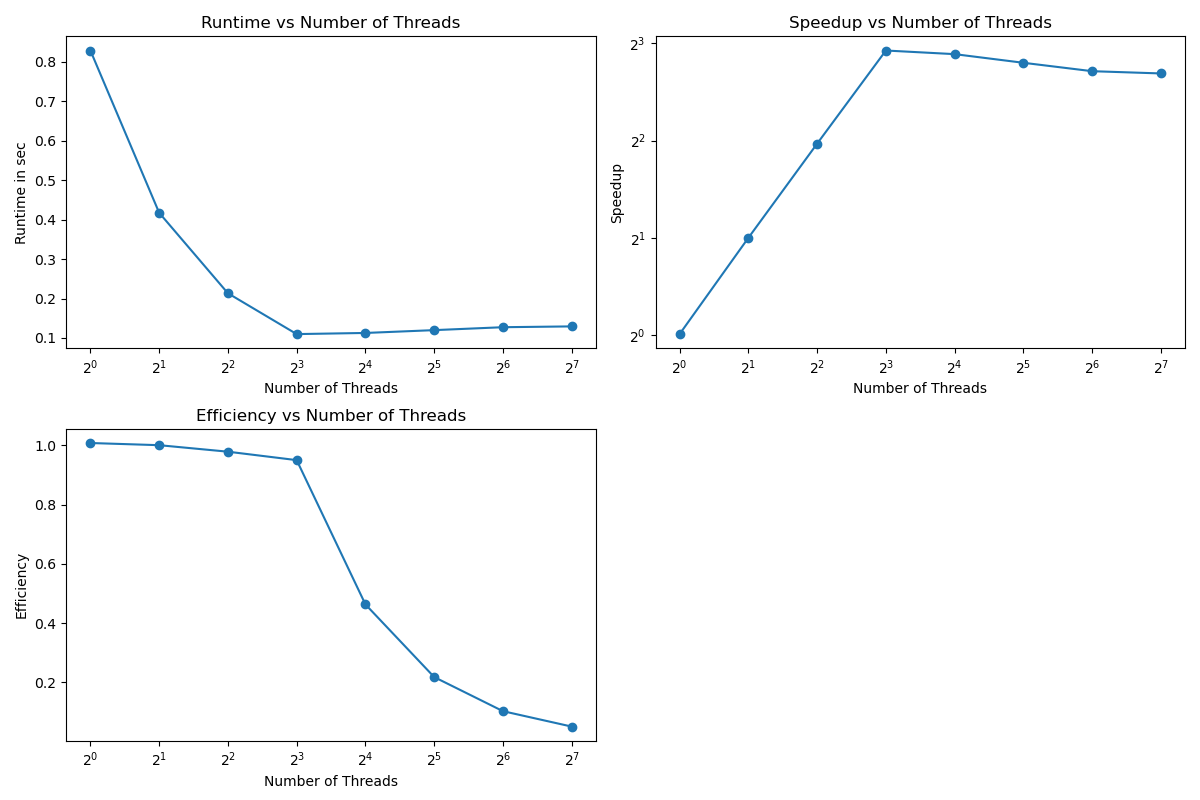
\includegraphics[width=0.9\textwidth]{./img/exe4/performance_analysis.png}
    \caption{Performance of the implementation}
\end{figure}

As we can observe, there is substantial improvement in the runtime of the program with the best runtime of 0.109891. 
However, the improvement is not meaningful after 8 threads which from 8 to 20 we can think of the Amdahl's law restriction
of non parallelizable part weighting more plus the overhead cost of the extra parallelization.
From 20 and more is even clearer since the maximum amount of cores is 20. In fact, is important to notice that I modified the 
given batch file since the required cores were 32, but we only have a maximum of 20 cores in Rosa cluster. 
The improvement in performance is almost ideal until 8 threads, then the performance gain is reduced because of the previously stated
reasons.

\section{Parallel loop dependencies with OpenMP \punkte{15}}
For achieving the desired improvement in runtime I tried several ideas.
One of them was to precompute an initial $opt[0]$ and $up$, $up^2$...$up^{n\_threads}$  
such that the following threads will compute on based on opt[0] as initial value and the different corresponding 
up as described in my following schema:


\begin{figure}[H]
    \centering
    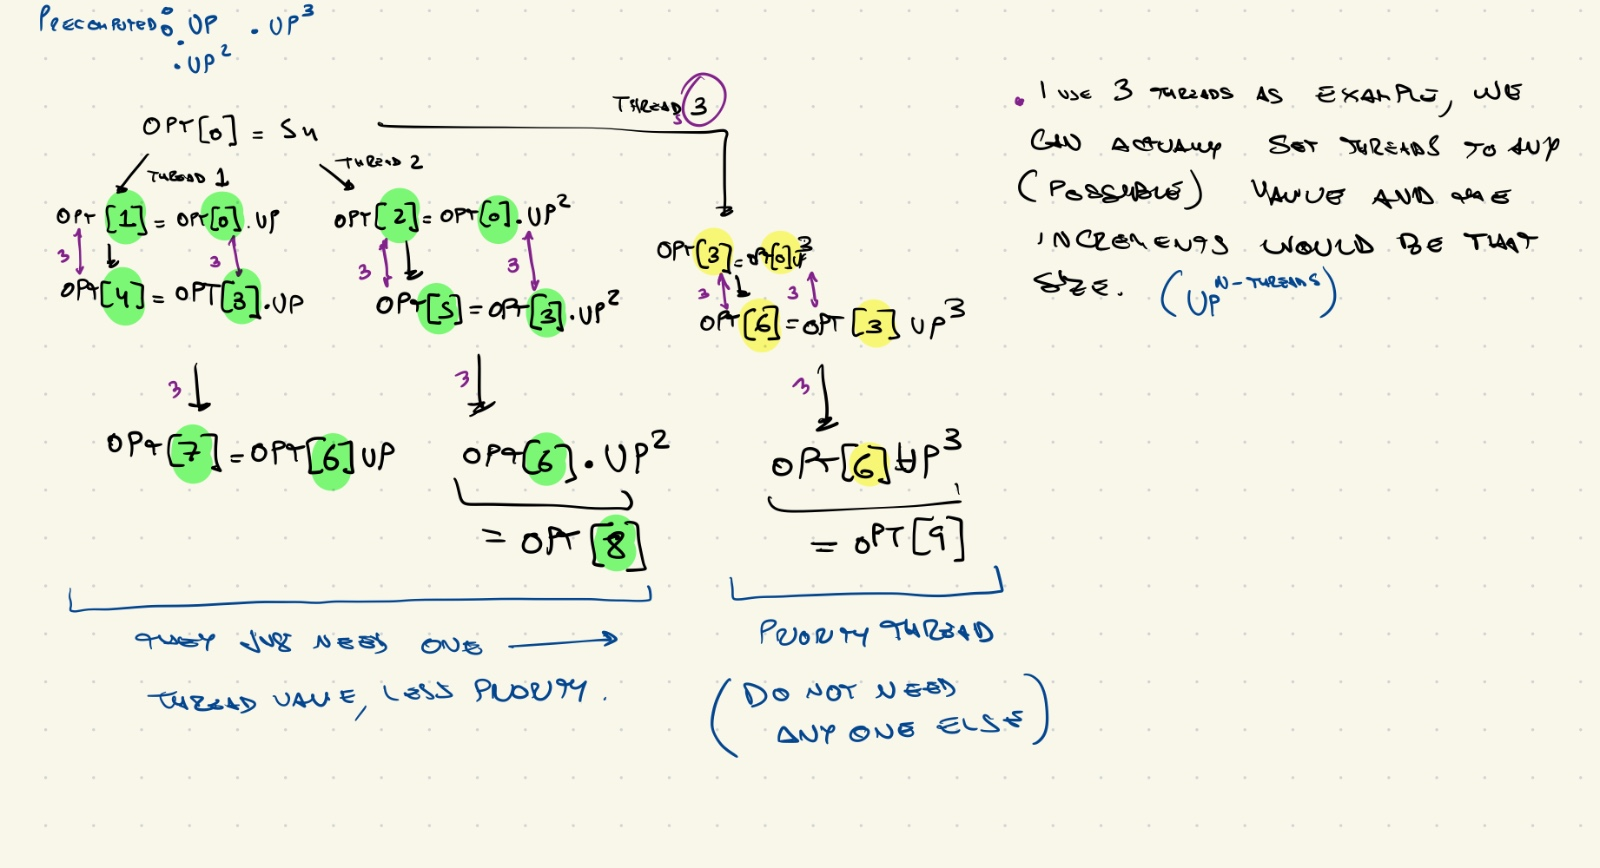
\includegraphics[width=0.9\textwidth]{./img/exe5/schema.jpeg}
    \caption{Idea for parallelization as tasks}
\end{figure}

The result of the biggest iteration among them will be the input of the other, therefore it will have
a priority as a task.
However, I was not able to parallelize this without a significant overhead cost. Despite this, 
this implementation without parallelization looks like a loop unrolling with a significant improvement in performance
with approximately 4.32 seconds of runtime in a node of Rosa cluster without any parallelization vs the 6.74 sec that it takes 
the basic sequential implementation.\footnote{The file name of the implementation is "recur\_omp\_unroll.cpp"}

Another idea, was to create different chunks for each thread to work on, with values precalculated to it. For this to work, we need to calculate the
starting value of each thread chunk of iterations before the loop and take advantage that we can fit the chunk on the cache memory. 
Then, each thread will use its precomputed to start its iterations and continue from there without any need of extra calculations. 
We first obtain the number of threads and compute how the chunk would be distributed since in static scheduling (we sadly relay on it)
the chunks are distributed evenly. Then, we precompute the chunk values form of the up powers to apply to each starting Sn.
We can reach such start value using this precomputed values and up, as an example with the given values:

Initial value $S_n = 1.00000001$
Multiplier $up = 1.00000001$

With CHUNK\_SIZE = 1024, our pattern chunk stores:
chunk[0] = 1.0 
chunk[1] = 1.00000001    ($up^1$)
chunk[2] = 1.00000002    ($up^2$)
...
chunk[1023] = 1.00001024 ($up^{1023}$)

chunk\_multiplier = chunk[1023] * up = $up^{1024}$

Therefore, with chunk\_multiplier: need only 2 multiplications (2048/1024 = 2 jumps)

Then, we simply need to compute the starting point of each chunk knowing the symmetry of omp for static scheduling.
And accounting for the remainder of values we could not "cover" with the chunks. We finally return the last value of Sn. 
The final running time of the implementation is 3.74 seconds, which is a significant improvement over the sequential implementation
and a bit better than the unrolling. \footnote{The file name of the implementation is "chunky.cpp"}

Lastly, I tried to implement the parallelization using firstprivate and lastprivate as given following a similar idea that before. 
Such that since each thread gets an equal chunk of the iterations, we can pass a counter and Sn as firstprivate where count gets the value 0 initially
for all threads and Sn the initial given value. Then, when the counter is 0 (the first iteration for each thread), we can compute the first value of the sequence that 
each thread needs to compute. Using, one time only, the pow function and the value of n at that moment. When that is done, we proceed with the sequence calculation as 
before, but now we have the initial value calculated for each thread and there is no dependency among them. However, I could not achieve with this implementation
a substantial increment in performance against the sequence implementation. Given that the use of pow initially in conjunction with parallelization overhead, 
I suspect, overpass the benefits of the parallelization.
\footnote{File name: recur\_omp\_private.cpp}

\section{Quality of the Report \punkte{15}}


\end{document}